\section{Quantum programming}

Quantum programming is setting up operations on quantum states in a specific order.

\subsection{Quantum Circuit}

To represent the operations done, their order and target states, one uses a quantum circuit. A single state, without any operations, in quantum circuit notation looks like the following

\begin{figure}[H]
    \centering
    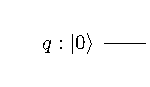
\includegraphics{Figures/Circuits/Theory/basecircuit.pdf}
\end{figure}

$q$ indicates in which bit of the registry the state resides and the line indicates what operations are done on the state, starting from left to right. So writing

$$H \ket{0}$$

in quantum circuit notation we have

\begin{figure}[H]
    \centering
    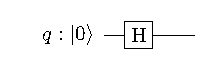
\includegraphics{Figures/Circuits/Theory/Hbasecircuit.pdf}
\end{figure}


Doing operations in a row, for example

$$\sigma_x  \sigma_yH \ket{0} \; ,$$

would be added to the right of the first Hadamard gate:

\begin{figure}[H]
    \centering
    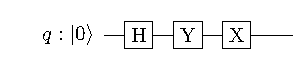
\includegraphics{Figures/Circuits/Theory/xyHbasecircuit.pdf}
\end{figure}

Some operations require a control. For the $\textbf{CNOT}$ gate we have the control marked by a $\Huge{\cdot}$ and the target qubit marked by $\oplus$ as shown here:

\begin{figure}[H]
    \centering
    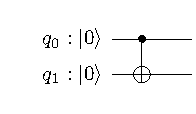
\includegraphics{Figures/Circuits/Theory/cxbasecircuit.pdf}
\end{figure}


\subsection{Measurement of Output}

In quantum mechanics we have that measuring a state changes it, or in our case the qubits collapses to either one of our base vectors $\ket{0}$ or $\ket{1}$. The measurement of a qubit on a quantum circuit is represented as the following:

\begin{figure}[H]
    \centering
    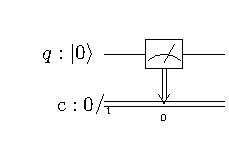
\includegraphics{Figures/Circuits/Theory/measurebasecircuit.pdf}
\end{figure}


Measuring here will either give us $\ket{0}$ or $\ket{1}$ with an equal $50\%$ chance. The information we want is most often the probabilities, and not the final state itself, since the probabilities ties to what state the qubit was in before it was measured. To extract the probabilities one utilizes the law of large numbers by computing the circuit a $N$ number of times and calculate the average number of $\ket{0}$ measurements and $\ket{1}$ measurements.

\subsection{Transformation of basis}

When measuring the qubits of a quantum circuit we are be often limited to doing the actual measuring in the z-basis. To overcome this limitation we simply transform the basis of the qubits to the basis we want to measure them in, or rather shift them back to the z-basis from the desired basis of measurement. The different basis transformations are as follows. \newline
\vskip 0cm
\textbf{Z-basis}:

\begin{figure}[H]
    \centering
    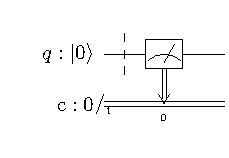
\includegraphics{Figures/Circuits/Theory/zm.pdf}
\end{figure}

Since we are already in the z-basis this one requires no transformation. The dashed line is to indicate that there are some sequence preceding it.
\newline\vskip 0cm
\textbf{X-basis}:

\begin{figure}[H]
    \centering
    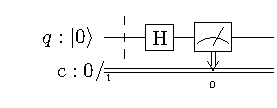
\includegraphics{Figures/Circuits/Theory/xm.pdf}
\end{figure}

which comes from the fact that

\begin{equation}
    HXH = Z \; .
\end{equation}

And similarly
\newline\vskip 0cm
\textbf{Y-basis}:

\begin{figure}[H]
    \centering
    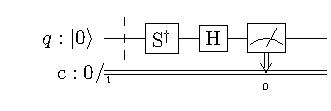
\includegraphics{Figures/Circuits/Theory/ym.pdf}
\end{figure}

where

\begin{equation}
    S^{\dagger}HYHS^{\dagger} = Z \; .
\end{equation}

\subsection{Circuit measurement to expectation value}

In the context of measurement the energy of a state for a given Hamiltonian we need to take into account the eigenvalues of the basis we measure in, here the z-basis. For the z-basis we have that

\begin{equation}
    Z\ket{0} = 1\ket{0} \;\;\;\;\;\;Z\ket{1} = -1\ket{1} \;,
\end{equation}

which means that for an example Hamiltonian

\begin{equation}
H_{\psi} = \varepsilon\sigma_x
\end{equation}

will have the expectation value

\begin{equation}
\left < H_{\psi} \right > = \varepsilon \left < \sigma_x \right > \; ,
\end{equation}

where

\begin{equation}
\left < \sigma_x \right > = n_0 - n_1 \; ,
\end{equation}

since we have matched it against the z-basis we measure in. Here $n_0$ and $n_1$ is the number of $\ket{0}$ and $\ket{1}$ measured respectively. For more than one qubit the eigenvalues accumulate. If we change our Hamiltonian to

\begin{equation}
H_{\psi} = \varepsilon\sigma_x \otimes \sigma_y \; ,
\end{equation}

we end up with the calculation of the expectation value

\begin{equation}
\left < \sigma_{x} \otimes \sigma_y \right > = n_{00} - n_{01} - n_{10} + n_{11}\; ,
\end{equation}

which can be generalized for $d\cdot n_s$ where $s$ is a basis state:

\begin{equation}
    d = (-1)^{N_1} \; ,
\end{equation}

where $N_1$ is the number of $1$'s in the basis state $s$.
